\section{\label{section:results}Numerical Results}
\begin{table}
  \centering
  \begin{tabular}{lll}
    Quantity                 & Symbol            & Value                        \\ \hline
    Speed of light           & $c$               & \SI{300}{\micro\meter \per \pico\second} \\
    Transition frequency     & $\omega_0$        & $\SI{1500}{\milli\eV}/\hbar$ \\
    Transition dipole moment & $\vb{d}$          & \SI{10}{\elementarycharge\bohr} (uniform) \\
    Decoherence times        & $T_{1}, T_{2}$    & \SIlist{10;20}{\pico\second} \\
    Laser frequency          & $\omega_L$        & $\SI{1500}{\milli\eV}/\hbar$ \\
    Laser wavevector         & $\vb{k}_L$        & $\omega_L/c$ ($\vb{k}_L \cdot \vb{d} = 0$) \\
    Pulse width              & $\sigma/\omega_L$ & \SI{1}{\pico\second} \\
    Pulse area               &  --               & $\pi$ \\
    %Number density          & $n$               & $< \SI{1.6e4}{\micro\meter\tothe{-3}}$ \\
    %\hline
    %Speed of light           & $c$            & \SI{299.792458}{\micro\meter\per\pico\second} \\
    %Reduced Planck constant  & $\hbar$        & \SI{0.65821193}{\milli\eV \pico\second} \\
    %Vacuum permeability      & $\mu_0$        & \SI{2.013e-4}{\milli\eV \pico\second\squared \per \elementarycharge \per \micro\meter}
  \end{tabular}
  \caption{\label{table:parameters}Simulation parameters (unless otherwise stated); \si{\elementarycharge} and \si{\bohr} denote the elementary charge and Bohr radius.
    The decoherence times here, while shorter than those typical of optical resonance experiments, afford a shorter computational time but preserve dynamical emission phenomena.
  }
\end{table}

Here we detail the results of investigations into coupled \qd{} behavior with the model presented thus far.
Our algorithm reliably handles tens of thousands of \qds{} and can simulate ten picoseconds of system dynamics in two days on a single processor.
We perform simulations of systems of \qds{} randomly distributed throughout a simulation volume experiencing a laser pulse of the form
\begin{equation}
  \tilde{\mathbf{E}}_L(\vb{r}, t) = \tilde{\mathbf{E}}_0 e^{-(\vb{k}_L \cdot \vb{r} - \omega_L t)^2/(2\sigma^2)}.
  \label{eq:pulse envelope}
\end{equation}
\Cref{table:parameters} provides the physical system parameters unless otherwise stated.

\subsection{Stability \& adjacency effects}

\begin{figure}
  \centering
  \conditionalFigureInput{figures/frame_comparison}
  \caption{
    Comparison of $\rho_{00}(t)$ using both fixed (requiring 59959 timesteps) and rotating (requiring 160 timesteps) reference frames for two interacting quantum dots.
    Both frames produce similar trajectories, however the inset spy reveals the fixed frame contains a minute oscilliatory term that the rotating frame does not.
  }
\end{figure}

\begin{figure}
  \centering
  \conditionalFigureInput{figures/density_stats}
  \caption{\label{fig:density stats}Population dynamics of adjacent \qds{} (top, shown with the trajectory of a \qd{} driven exclusively by the external laser in black) and a 1024-particle neighborhood (dots (1) and (2) maintain their separation and orientation between simulations).
    The interaction between particles gives a greatly diminished response to the external pulse through a dynamical detuning of the two-dot system.
    The majority of the neighboring particles in the 1024-dot system follow trajectories nearly identical to that prescribed by the laser (omitted for clarity); many-dot effects, however, produce significant oscillatory modes in the evolution of selected \qds{} (shown in gray).
    Note that $\rho_{00}^{\qty(1)}$ and $\rho_{00}^{\qty(2)}$ appear to have \emph{two} coherent modes in the presence of multiple dots: a high-frequency oscillation between the pair, as well as a low-frequency oscillation of the group about a decaying envelope.
}
\end{figure}

\Cref{fig:density stats} details $\rho_{00}(t)$ for two-, and 1024-particle simulations shown against a solution of \cref{eq:rotating liouville} for a \qd{} evolving according to $\tilde{\vb{E}}_L(\vb{r}, t)$ alone.
The system in \cref{fig:density stats}(a) contains two \qds{} with a separation of \SI{6.3}{\nano\meter} perpendicular to their mutual $\vb{d}$ to ensure large contributions from the near-field term of \cref{eq:radiated envelope}.
The two \qds{} in this system follow the same trajectory and both excite far less than either would in response to the incident laser alone.
These signatures indicate the effect arises as a dynamical frequency shift that brings adjacent \qds{} out of resonance with the applied electric field.
We note that this suppression effect occurred to varying degrees for all near-field arrangements of two \qds{} that we investigated.
In \cref{fig:density stats}(b), the system contains the same two-dot arrangement as in (a), however we have added an additional 1024 \qds{} randomly distributed throughout a $\SI{6.4e-2}{\micro\meter\cubed}$ cube centered around the original pair.
Most of these additional \qd{} populations deviate little from those produced by the laser-only pulse due to the large separation between particles.
Nevertheless, as we have filled the cube randomly, some regions of the system contain localized clusters of \qds{} that produce the suppression effect detailed above (for two adjacent particles) or populations with higher frequency oscillations (in the case of clusters with three or more \qds{}).
Specifically, the two ``original'' \qds{} acquire an out-of-phase oscillation with respect to each other as well as a lower frequency in-phase oscillation of the pair about a decaying envelope.


\begin{figure}
  \centering
  \conditionalFigureInput{figures/visit}
  \caption{\label{fig:nearfield box}Spatial distribution of $\abs{\tilde{\rho}_{01}}$ for 1024 \qds{} as an indicator of polarization.
    Recorded at $t = \SI{2}{\pico\second}$ relative to the peak of a \SI{1}{\pico\second}-wide $\pi$-pulse, the color and size of each sphere indicates the location of each \qd{} and its polarization.
    Following a $\pi$-pulse, a single \qd{} would have no remnant polarization; here, due to the near-field interactions between particles, clusters of \qds{} remain in highly-polarized states depending on their separation.
  }
\end{figure}

\begin{figure}
  \centering
  \conditionalFigureInput{figures/visit_ipr}
  \caption{\label{fig:ipr}Inverse participation ratio (IPR) for the system shown in \cref{fig:nearfield box}. The dashed line indicates the sample time for \cref{fig:nearfield box}.}
\end{figure}

\Cref{fig:nearfield box} further illustrates the near-field coupling between \qds{}.
Here, 1024 \qds{} randomly fill an \SI{8e-3}{\micro\meter\cubed} cube and the same \SI{1}{\pico\second} Gaussian $\pi$-pulse illuminates the system.
Without any inter-dot interactions, such a pulse would perfectly transition every \qd{} from $\ket{0}$ to $\ket{1}$, leaving behind no polarization after the pulse has passed.
As the system in \cref{fig:nearfield box} has experienced most of the pulse, the majority of the \qds{} behave this way.
A number of particles remain polarized well after the pulse has passed through the system, however, due to their apparent proximity.

\subsection{Polarization enhancement}

Borrowing from standard measures of localization (in which one calculates integrals of $\vb{E}$ over the simulation volume), we have adapted the inverse participation ratio (IPR)  of the dot polarization as
\begin{equation}
  \text{IPR}(t) = \frac{\sum_\ell \abs{\tilde{\vb{p}}_\ell(t)}^4}{\qty(\sum_\ell \abs{\tilde{\vb{p}}_\ell(t)}^2)^2}
  \label{eq:ipr}
\end{equation}
to provide a quantitative description of these phenomena~\cite{Schwartz2007}.
\Cref{fig:ipr} shows this quantity for the system in \cref{fig:nearfield box}.
The maximum IPR occurs some time after the pulse has passed through the system, indicating strongly-coupled \qds{} retain their polarization longer than their neighbors.
Moreover, this dynamical localization effect features oscillations which suggests many-dot effects contribute to the dynamics within a narrow spectral region.

\begin{figure*}
  \centering
  \subfloat{
    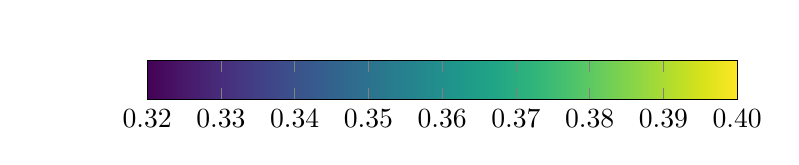
\begin{tikzpicture}
      \node (spacer) at (-1.4, 0) {};
      \begin{axis}[
        hide axis,
        scale only axis,
        height=0pt,
        width=0pt,
        colormap/viridis,
        colorbar horizontal,
        point meta min=0.32,
        point meta max=0.40,
        colorbar style={
          width=0.6180339887\textwidth,
          xtick={0.32, 0.33, 0.34, 0.35, 0.36, 0.37, 0.38, 0.39, 0.40},
          xticklabels={$\leqslant 0.32$, $0.33$, $0.34$, $0.35$, $0.36$, $0.37$, $0.38$, $0.39$, $0.40 \leqslant$},
        }
      ]
      \addplot [draw=none] coordinates {(0,2)};
      \end{axis}
    \end{tikzpicture}
  } \\
  \subfloat{
    \begin{tikzpicture}[>=Latex]
      \node[] (tube0) at (0,-1) {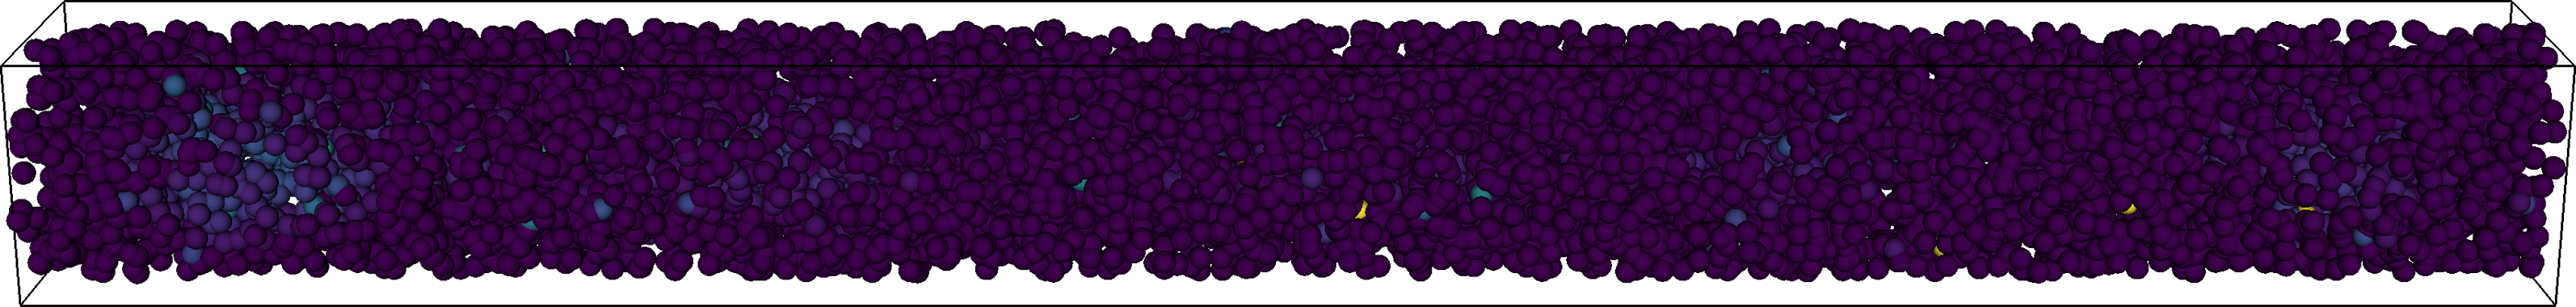
\includegraphics[width=0.95\textwidth]{figures/tube/tube_print_0.png}};
      \node[] (tube1) at (0,-3) {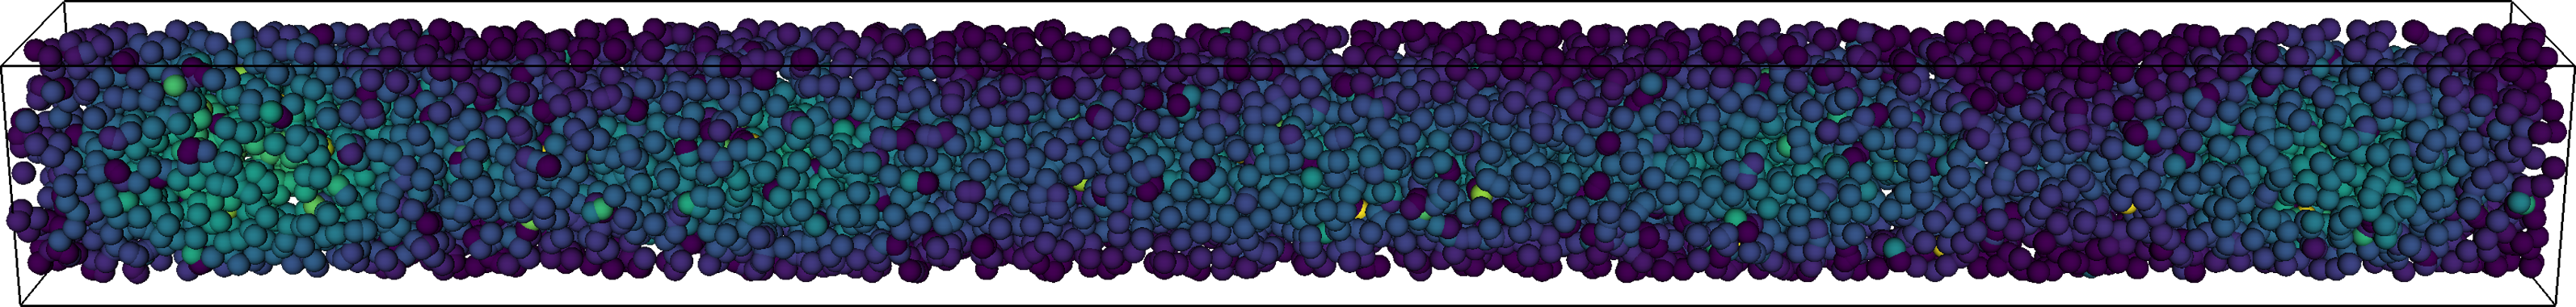
\includegraphics[width=0.95\textwidth]{figures/tube/tube_print_1.png}};
      \node[] (tube2) at (0,-5) {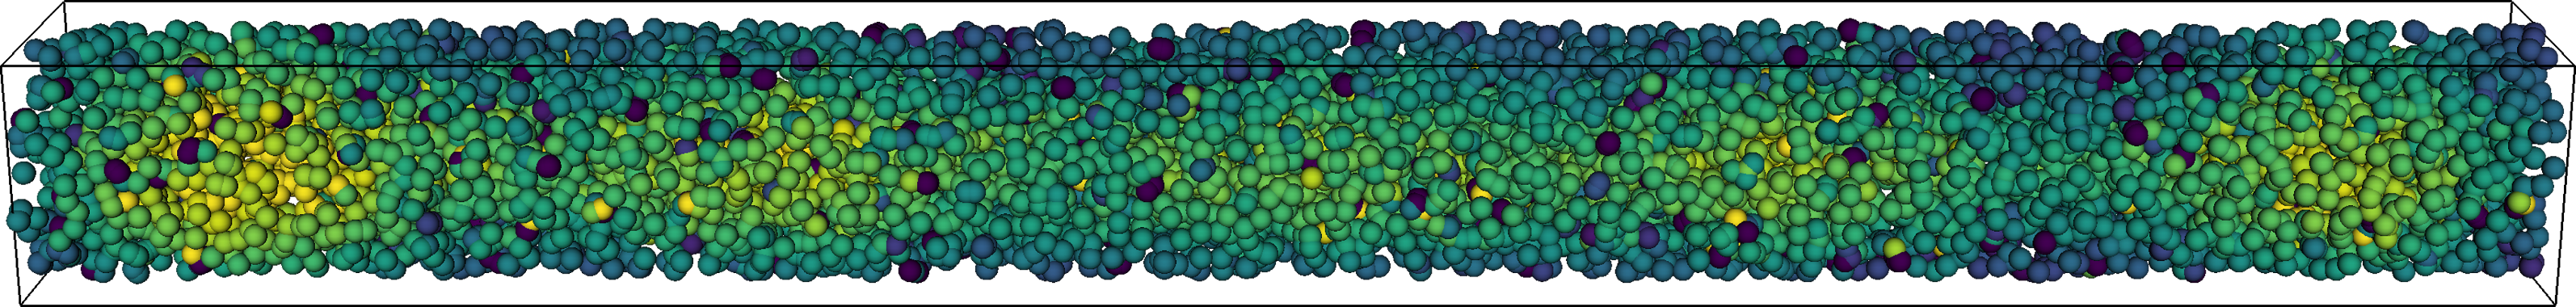
\includegraphics[width=0.95\textwidth]{figures/tube/tube_print_2.png}};
      \node[] (tube3) at (0,-7) {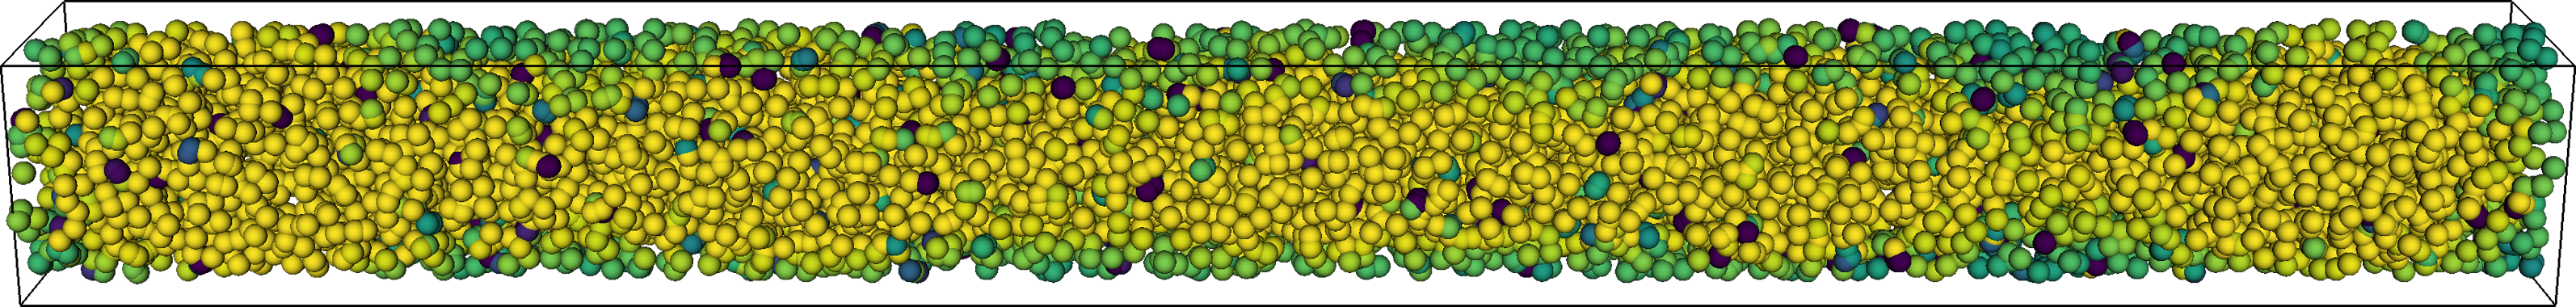
\includegraphics[width=0.95\textwidth]{figures/tube/tube_print_3.png}};

      \draw[->,thick] ($(tube0.west) - (0.3,0)$) -- ($(tube3.west) - (0.3,0)$) node[midway,fill=white, rotate=90] {Time};
      \draw[->,thick] ($(tube3.south east) - (3,0.3)$) -- ($(tube3.south east) - (0,0.3)$) node[midway,fill=white] {$\vu{k}$};
    \end{tikzpicture}
  }
  \caption{\label{fig:tubes}
    Coloration of $\abs{\tilde{\rho}_{01}}$ as an indicator of $\abs{\vb{\tilde{P}}}$ at $t_1 = \SI{-0.05}{\pico\second}$, $t_2 = \SI{0}{\pico\second}$, $t_3 = \SI{0.05}{\pico\second}$, and $t_4 = \SI{0.10}{\pico\second}$ relative to the peak of a \SI{1}{\pico\second}-wide pulse.
    \num{10000} \qds{} randomly distributed throughout a $\SI{0.2}{\micro\meter} \text{ (radius)} \times \SI{4}{\micro\meter}$ cylinder oriented along $\vb{k}_L$ demonstrate near-field the effects of \cref{fig:density stats} as distinct, outlying bright/dark \qds{}.
    Additionally, the size of the system allows for wavelength-scale phenomena that appear here as five standing regions of enhanced polarization.
    (Note that we model \qds{} as point objects; the size of the spheres here has no physical interpretation.)
  }
\end{figure*}

\Cref{fig:tubes} depicts the evolution of $\abs{\rho_{01}(\vb{r})}$ as an indicator of $\tilde{\vb{P}}$ for a cylinder containing \num{10000} \qds{}.
The cylinder has a radius of \SI{0.2}{\micro\meter} and a length of \SI{4}{\micro\meter}, and the incident $\vb{k}_L$ lies along the cylindrical axis (again perpendicular to $\vb{d}$ so as to maximize the long-distance interaction between \qds{}).
This simulation captures the suppression effects of \cref{fig:density stats,fig:nearfield box} as a small number of \qds{} remain in an unexcited state while the cylinder polarizes around them.
Additionally, due to the length of the cylinder, larger regions of enhanced polarization begin to appear as the system polarizes---an effect we did not observe in sub-wavelength structures.
We liken these nodes to standing waves in a cavity that arise from the far-field interaction term of \cref{eq:radiated envelope}.
As the pulse varies little over the length of the cylinder, identical simulations run without interactions (i.e.~$\mathcal{Z} = 0$ everywhere) produce homogeneous polarization distributions.
Reducing the simulation to a planar geometry (\cref{fig:wide plate}) preserves both the short-range (dark, adjacent \qds{}) and long-range (regions of enhanced/diminished polarization) phenomena observed in \cref{fig:tubes}.
We note these geometries produce a much weaker effect than their fully three dimensional counterparts, though larger simulations with greater far-field contributions or \qds{} engineered to have a larger dipole moment may produce more measurable effects.

\begin{figure}
  \centering
  \begin{tikzpicture}[>=latex]
    \begin{axis}[
        xtick scale label code/.code={$\cdot \lambda$},
        enlargelimits=false,
        axis equal image,
        colormap/viridis,
        colorbar horizontal,
        point meta min=0.46,
        point meta max=0.47,
        colorbar style={
          xtick={0.461, 0.463, 0.465, 0.467, 0.469},
          xticklabels={$\leqslant 0.461$, 0.463, 0.465, 0.467, $0.469 \leqslant$},
          at={(0,1.5)},
          anchor=north west,
        }
      ]
      \addplot graphics [xmin=0,xmax=3,ymin=0,ymax=1] {figures/wide_plate.png};
      \draw[->, white, thick] (axis cs:2.25,0.8) -- (axis cs:2.75,0.8) node[at end, anchor=west] (A) {$\vu{k}$};
    \end{axis}
  \end{tikzpicture}
  \caption{\label{fig:wide plate}
    Coloration of $\abs{\tilde{\rho}_{01}}$ for \num{10000} \qds{} arranged in a finite planar geometry (in units of $\lambda$).
    The slab displays a prominent polarization pattern \SI{1.25}{\pico\second} after the peak of a \SI{1}{\pico\second} pulse.
  }
\end{figure}

\subsection{Inhomogeneous broadening}

\begin{figure*}
  \centering
  \conditionalFigureInput{figures/inhomogeneous/inhomog_aggregate.tex}
  \caption{\label{fig:broadened} 
    $z$-distribution of polarization $\abs{\tilde{\rho}_{01}}$ for the geometry in \cref{fig:tubes}.
    In each simulation, \num{10000} \qds{} had random Gaussian noise (with width parameters of \SIlist{0.0;0.2;0.4;0.6}{\milli\eV}) added to a resonant $\hbar \omega_0 = \SI{1500}{\milli\eV}$.
    The induced long-range patterns in the polarization remain for mild detunings $\lesssim \SI{0.5}{\milli\eV}$ but have completely washed out at \SI{0.6}{\milli\eV}.
    Additionally, each simulation displayed the characteristic near-field coupling effects of \cref{fig:density stats} (not visible here).
  }
\end{figure*}

Thusfar we have investigated only homogeneous systems (i.e. an identical $\omega_0$ for every \qd{} in the system).
To probe the effects of interaction-independent inhomogeneities (possibly occurring due to some experimental variation in \qd{} sizes), \cref{fig:broadened} presents four simulations with normally-distributed transition frequencies characterized by a width parameter.
In simulations with mild detuning, we observe a distribution pattern characteristic of the enhancement phenomenon seen in \cref{fig:tubes}.
More variation in the detuning distribution, however, quickly serves to destroy these phenomena leaving only ``pulse-driven'' effects.
At present, inhomogeneous broadening in \qds{} typically exceeds the values used in \cref{fig:broadened}.
Impurity-bound excitons have greatly diminished inhomogeneous effects and thus could offer an avenue to observe these phenomena~\cite{Thewalt1977}.
